\pagenumbering{arabic}
\setcounter{page}{1}

\section{Métrica na Esfera}

%%%%%%%%%%%%%%%%%%%%%%%%%%%%%%%%%%%%%%%%%%%%%%%%%%%%%%%%%%%%%%%%%%%%%
\subsection{Projeção Estereográfica}


Definindo um sistema de coordenadas cartesiano, temos que para uma 
esfera, $S^2\subset\R^3$, com centro na origem, e de raio R, sua 
equação é dada, em coordenadas cartesianas, pela equação: 
%
\begin{equation}
x^2 + y^2 + z^2 = R^2.
\end{equation}
%
Para fazer uma descrição local, na esfera, deve-se utilizar um 
sistema de coordenadas esféricas, $(r,\theta,\varphi)$, de modo que 
para a esfera tenhamos sempre $r = R$, dessa maneira as coordenadas 
locais $(\theta,\varphi)$, para pontos na superfície da esfera,  
%
\begin{equation}
0 \leq \theta \leq \pi \ \, \ \ 0 \leq \varphi \leq 2\pi.
\end{equation}
%
Devido à troca de coordenadas, cartesianas para esféricas, surgem 
pontos singulares na esfera, sendo estes o polo norte, $\theta = 0$, e 
o polo sul, $\theta = \pi$. A métrica cartesiana tem a seguinte forma:
%
\begin{equation}
ds^2 = \sum_{i}g_{ij}dx^i dx^j = dx^2 + dy^2 + dz^2, 
\end{equation}
%
lembrando que para a métrica cartesiana, tem-se, $g_{ij} = \delta_{ij}$, 
onde $\delta_{ij}$, é o delta de Kronecker. Utilizando as transformações 
de  coordenadas, $x^i = x^i(y^j)$, de cartesianas para esféricas,
%
\begin{align}
x &= r\sin\theta\cos\varphi \\ 
y &= r\sin\theta\sin\varphi \\
z &= r\cos\theta. 
\end{align}
%
Encontra-se a seguinte relação para a métrica, em coordenadas esféricas:
%
\begin{align}
\nonumber ds^2 &= dx^2 + dy^2 + dz^2 \\
               &= dr^2 + r^2(d\theta^2 + \sin^2\theta d\varphi^2)
\end{align}
%
Para a esfera, temos que $r = R$, logo $dr = 0$, e a métrica em 
coordenadas esféricas toma a seguinte forma: 
%
\begin{equation}
ds^2 = R^2(d\theta^2 + \sin^2\theta d\varphi^2). 
\end{equation}
%
A projeção estereográfica projeta um ponto $(\theta,\varphi)$, na esfera, 
em um ponto $(\rho,\varphi)$, no plano. Tomando um corte na seção 
transversal da esfera, em qualquer um de seus diâmetros, temos um 
círculo, de mesmo diâmetro que a esfera. Traçando uma reta que intercepta 
essa circunferência em dois pontos no círculo, em um ponto em um dos dois 
pólos e em um ponto genérico da circunferência, $P = (\theta,\varphi)$, 
e em um no plano xOy, $Q = (\rho,\varphi)$, temos uma projeção estereográfica.

Para encontrar uma relação entre os dois sistemas de coordenadas, podemos 
perceber logo de cara que, $\varphi = \varphi$, em ambos os sistemas, 
para encontrar $\rho = \rho(\theta)$, basta traçarmos um raio vetor, 
da origem até o ponto P na esfera/circunferência, determinando o ângulo 
$\theta$, entre o eixo Oz e o raio vetor.

Traçando uma reta que passa pela origem, e intercepta a esfera, tendo 
como reta suporte a reta da projeção estereográfica, pode-se perceber 
que esta reta é a altura, bissetriz e mediana do triângulo retângulo 
formado, de modo que o ângulo $\theta$ seja dividido em dois (bissetriz). 
Ver figura abaixo:

\begin{figure}[!ht]
 \centering
 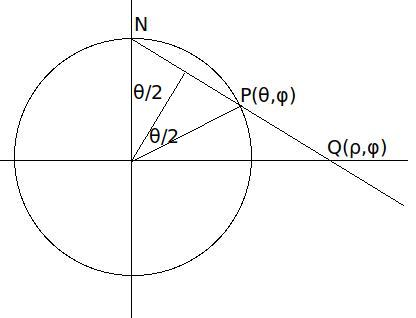
\includegraphics[scale=.60]{projecaoest1.jpeg}
 \caption{Projeção Estereográfica de um ponto, $(\theta,\varphi)$, 
 					da esfera, no plano, em um ponto, $(\rho,\varphi)$.}
 \label{projecao1}
\end{figure}

A partir da figura \ref{projecao1}, deve-se destacar o triângulo 
$\triangle ONQ$, veja a figura abaixo, onde é mostrado que o ângulo 
entre a reta traçada a partir do polo norte, N, até o plano xOy, 
e o eixo O$\rho$ é tal que seja igual à $\theta/2$, de modo que 
tenhamos a seguinte relação, $\rho = R\cot(\theta/2)$.

\begin{figure}[!ht]
 \centering
 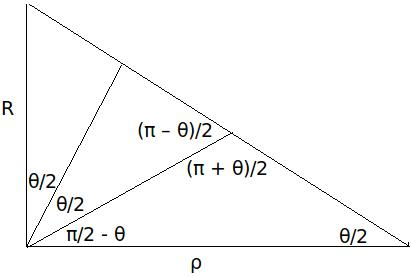
\includegraphics[scale=.5]{projecaoest2.jpeg}
 \caption{Ilustração que mostra a relação $\rho = R\cot(\theta/2)$.}
\end{figure}

Derivando a relação $\rho = R\cot(\theta/2)$, encontra-se,
%
\begin{align}
\nonumber d\rho &= - \frac{R}{2}\csc^2(\theta/2)d\theta \\ 
                &= - \frac{R}{2}(1 + \cot^2(\theta/2))d\theta,
\end{align}
%
De modo que tem-se a seguinte relação:
%
\begin{equation}
d\theta^2 = \frac{4R^2}{(R^2 + r^2)^2}d\rho^2,
\end{equation}
%
Tendo em conhecimento de que
%
\begin{equation}
\sin\theta = 2\sin(\theta/2)\cos(\theta/2),
\end{equation}
%
tem-se que:
%
\begin{equation}
\sin(\theta/2) = \frac{2\cot(\theta/2)}{1 + \cot^2(\theta/2)},
\end{equation}
%
Lembrando que $\rho = R\cot(\theta/2)$, tem-se o seguinte resultado:
%
\begin{equation}
\sin(\theta/2) = \frac{2R\rho}{R^2 + \rho^2},
\end{equation}
%
Inserindo os resultados encontrados para $d\theta^2$, $\sin^2(\theta/2)$, 
na na métrica da esfera, $ds^2 = R^2(d\theta^2 + \sin^2\theta d\varphi^2)$, 
encontra-se a seguinte relação para a métrica, no sistema de coordenadas 
da projeção estereográfica, $(\rho,\varphi)$:
%
\begin{align}
\nonumber ds^2 &= R^2(d\theta^2 + \sin^2\theta d\varphi^2) \\
               &= \frac{4R^4}{(R^2 + \rho^2)^2}(d\rho^2 + 
     \rho^2 d\varphi^2).
\end{align}
%
Lembrando que tem-se a seguinte relação, $\rho^2 = x^2 + y^2$, e de que, 
$x = \rho\cos\varphi$ e $y = \rho\sin\varphi$, vale a seguinte relação 
entre os sistemas de coordenada $(\rho,\varphi)$ e $(x,y)$:
%
\begin{equation}
dx^2 + dy^2 = d\rho^2 + \rho^2 d\varphi^2.
\end{equation}
%
Que nada mais é do que a transformação de coordenadas cartesianas para 
coordenadas polares. Dessa maneira tem-se que:
%
\begin{align}
\nonumber ds^2 &= R^2(d\theta^2 + \sin^2\theta d\varphi^2) 
\\ 
               &= \frac{4R^4}{(R^2 + \rho^2)^2}(dx^2 + dy^2)
\end{align}
%
De forma que, para encontrar a métrica da esfera, basta multiplicar 
a métrica do plano, $ds^2 = dx^2 + dy^2$, pela seguinte função:
%
\begin{equation}
f(\rho,R) = \frac{4R^4}{(R^2 + \rho^2)^2}.
\end{equation}
